

\begin{frame}
  \frametitle{Degradation Rate Base Case II}
  Base Case II : If the degradation rates for all pieces are 10\% per timestep 
  except the buffer. If five waste forms are necessary, the far field should 
  recieve no material within the 100 timesteps.

  \begin{figure}[htbp!]
    \begin{center}
      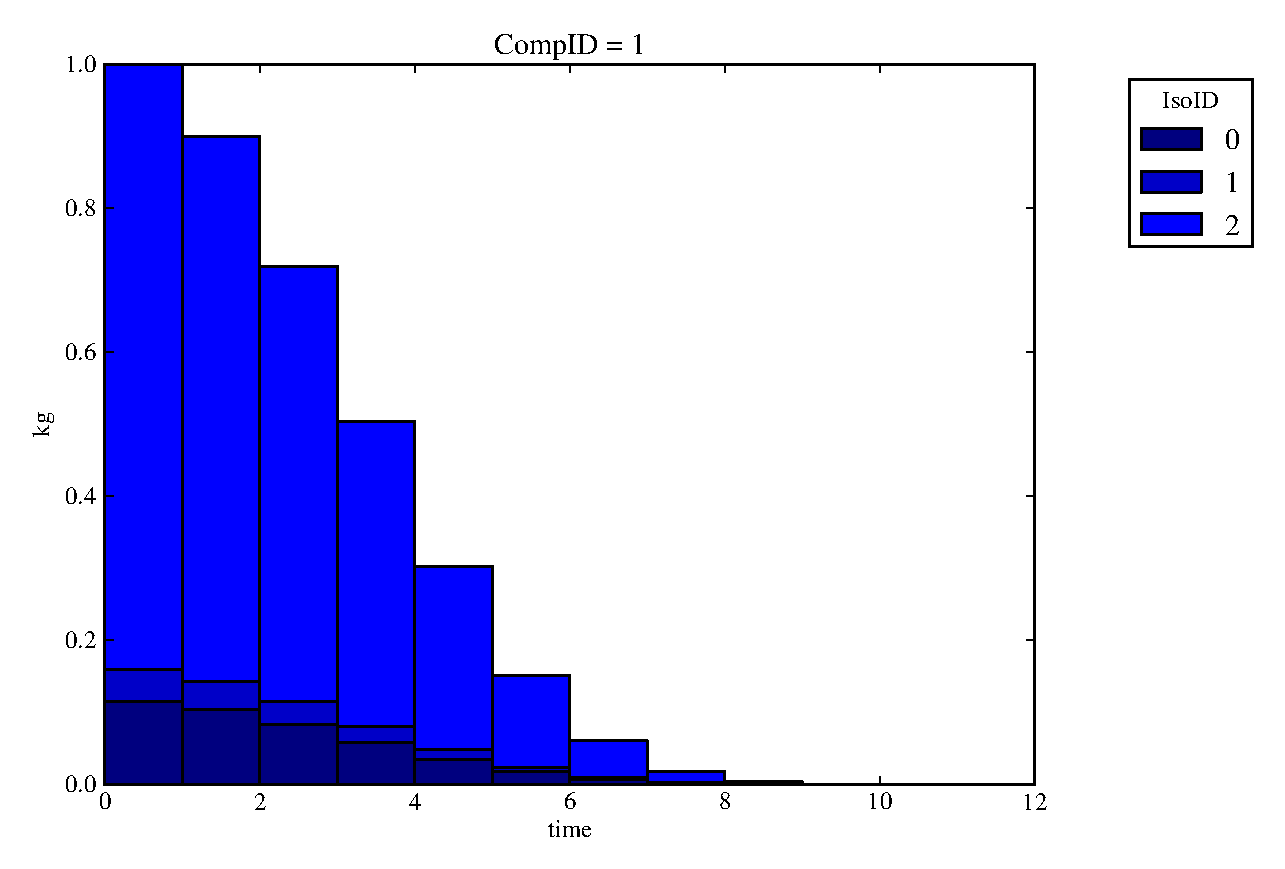
\includegraphics[width=0.2\textwidth]{cyder/images/buff0deg1.eps}
      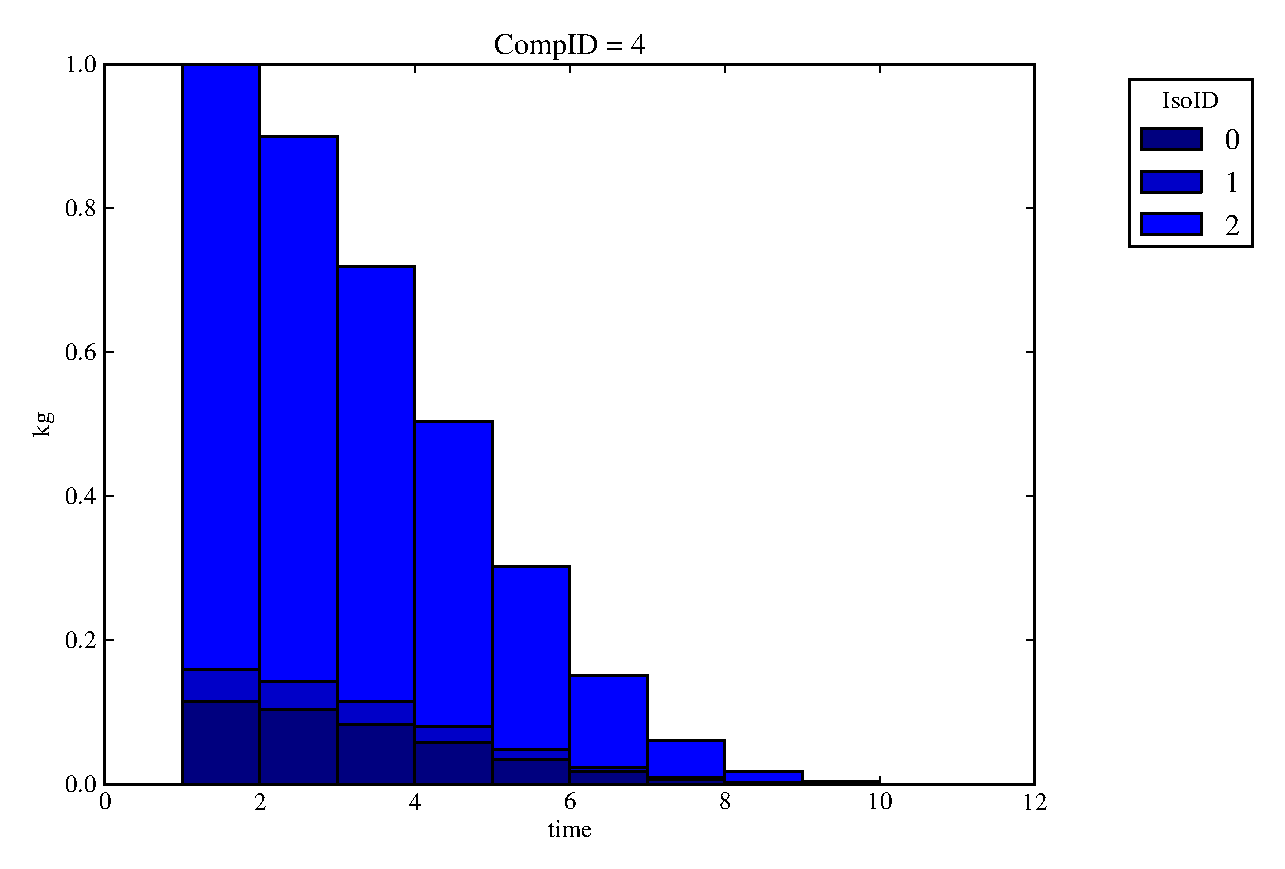
\includegraphics[width=0.2\textwidth]{cyder/images/buff0deg4.eps}
      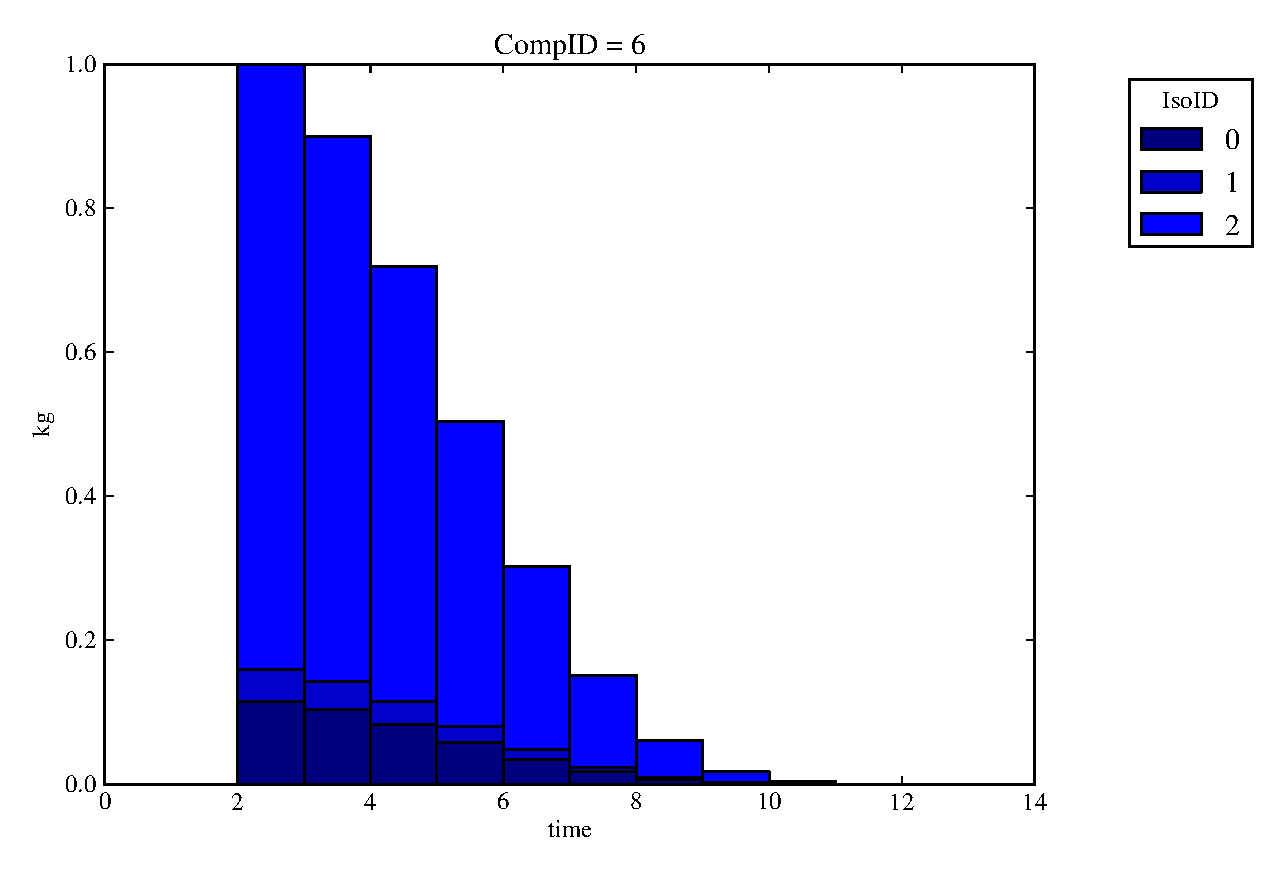
\includegraphics[width=0.2\textwidth]{cyder/images/buff0deg6.eps}
      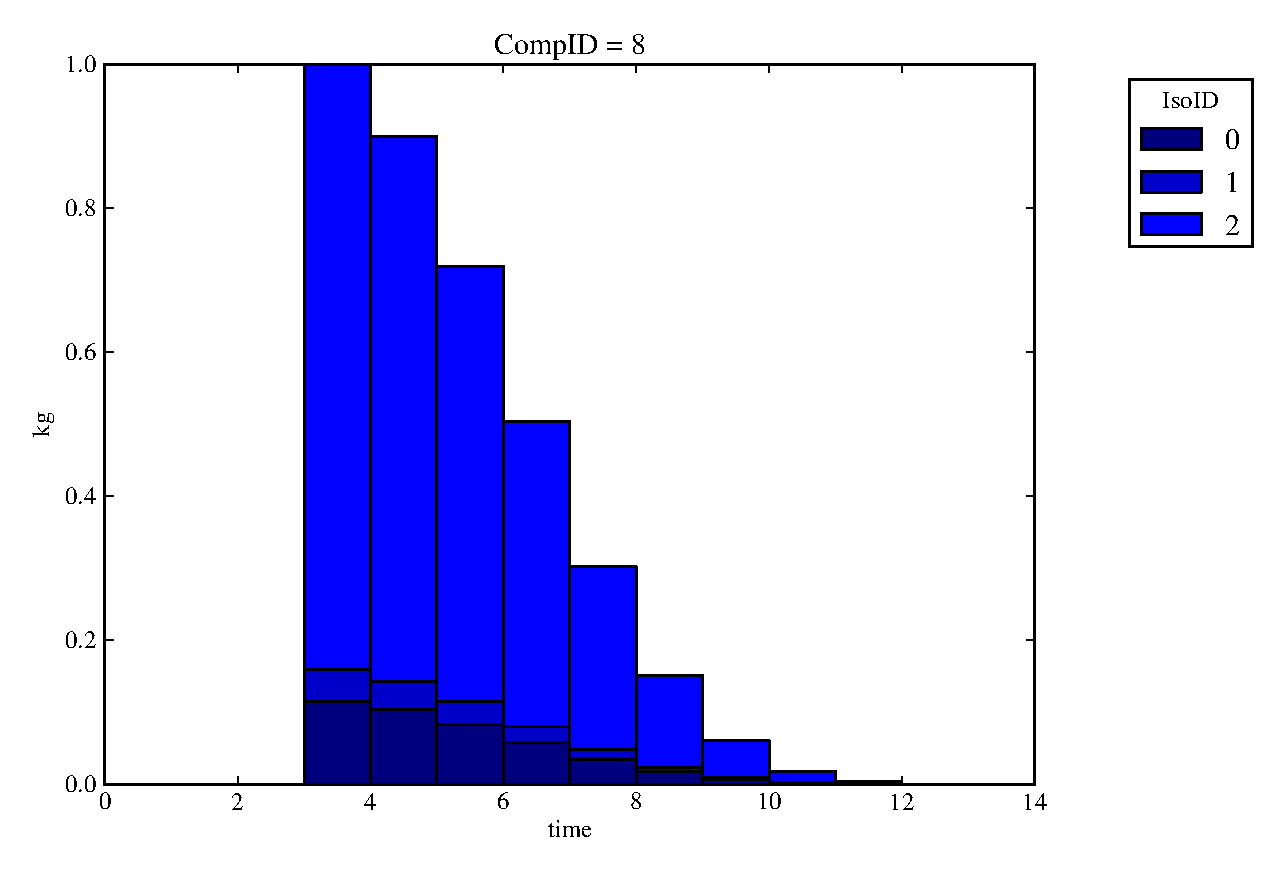
\includegraphics[width=0.2\textwidth]{cyder/images/buff0deg8.eps}
      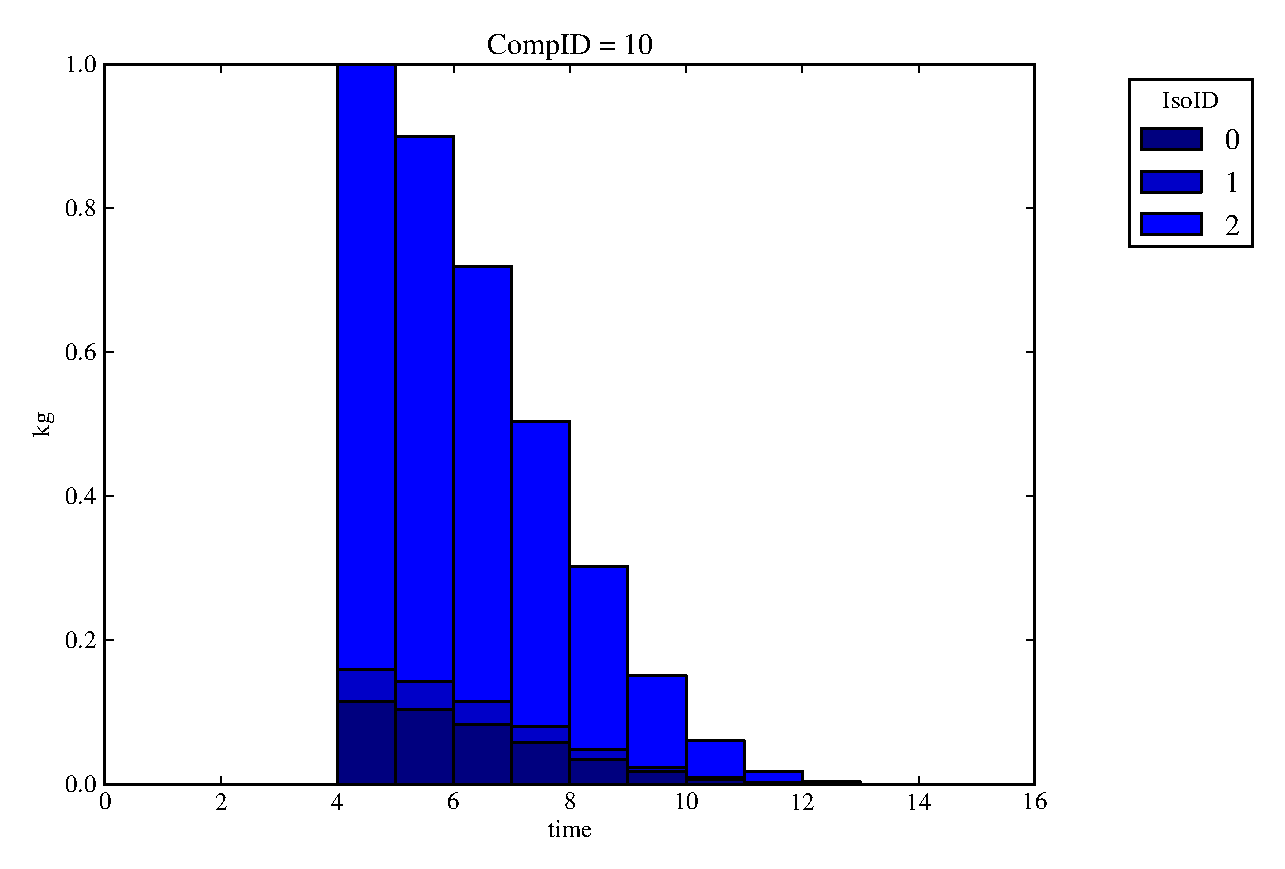
\includegraphics[width=0.2\textwidth]{cyder/images/buff0deg10.eps}
    \end{center}
  \end{figure}
\end{frame}

\begin{frame}
  \frametitle{Degradation Rate Base Case II}
  Base Case II : If the degradation rates for all pieces are 10\% per timestep 
  except the buffer. If five waste forms are necessary, the far field should 
  recieve no material within the 100 timesteps.

  \begin{figure}[htbp!]
    \begin{center}
      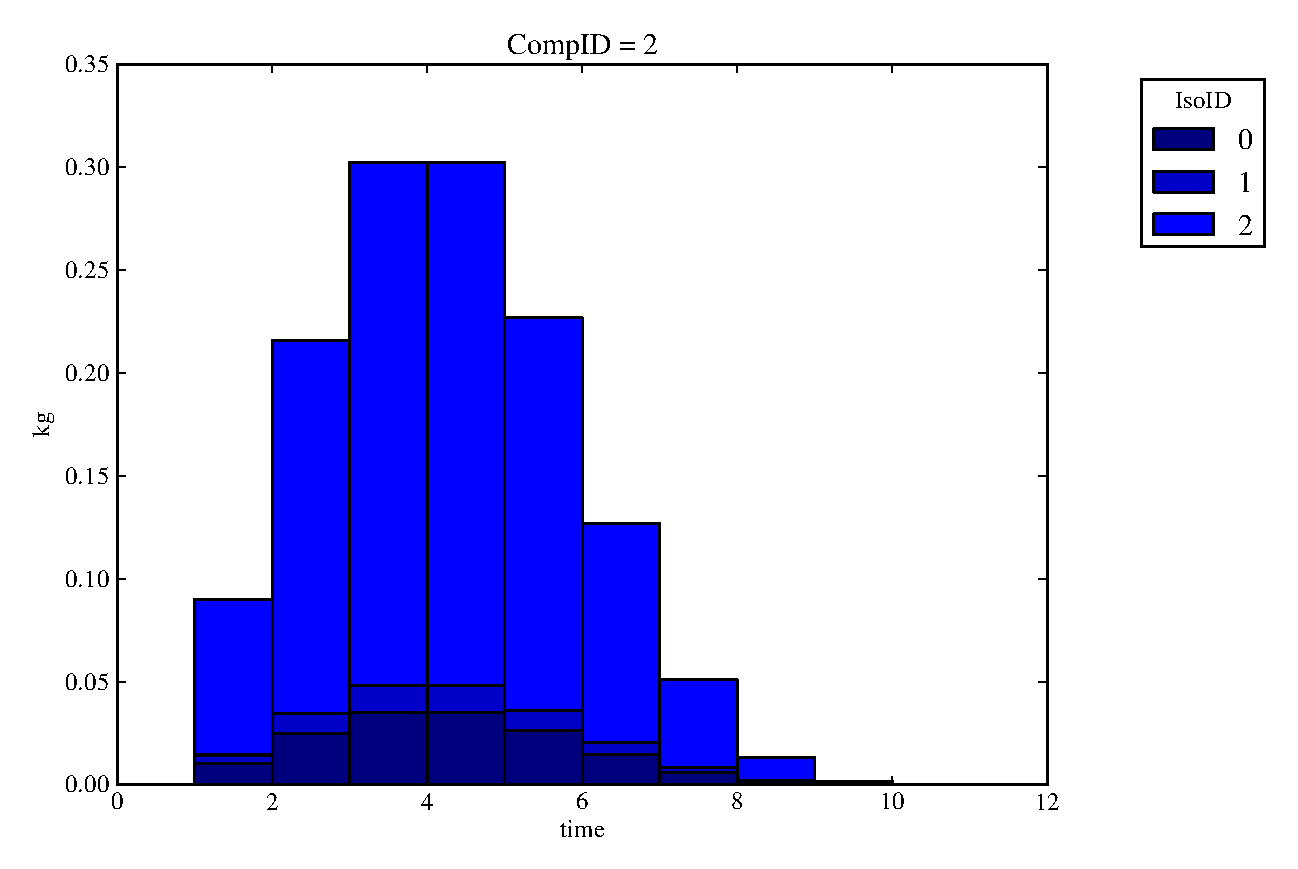
\includegraphics[width=0.2\textwidth]{cyder/images/buff0deg2.eps}
      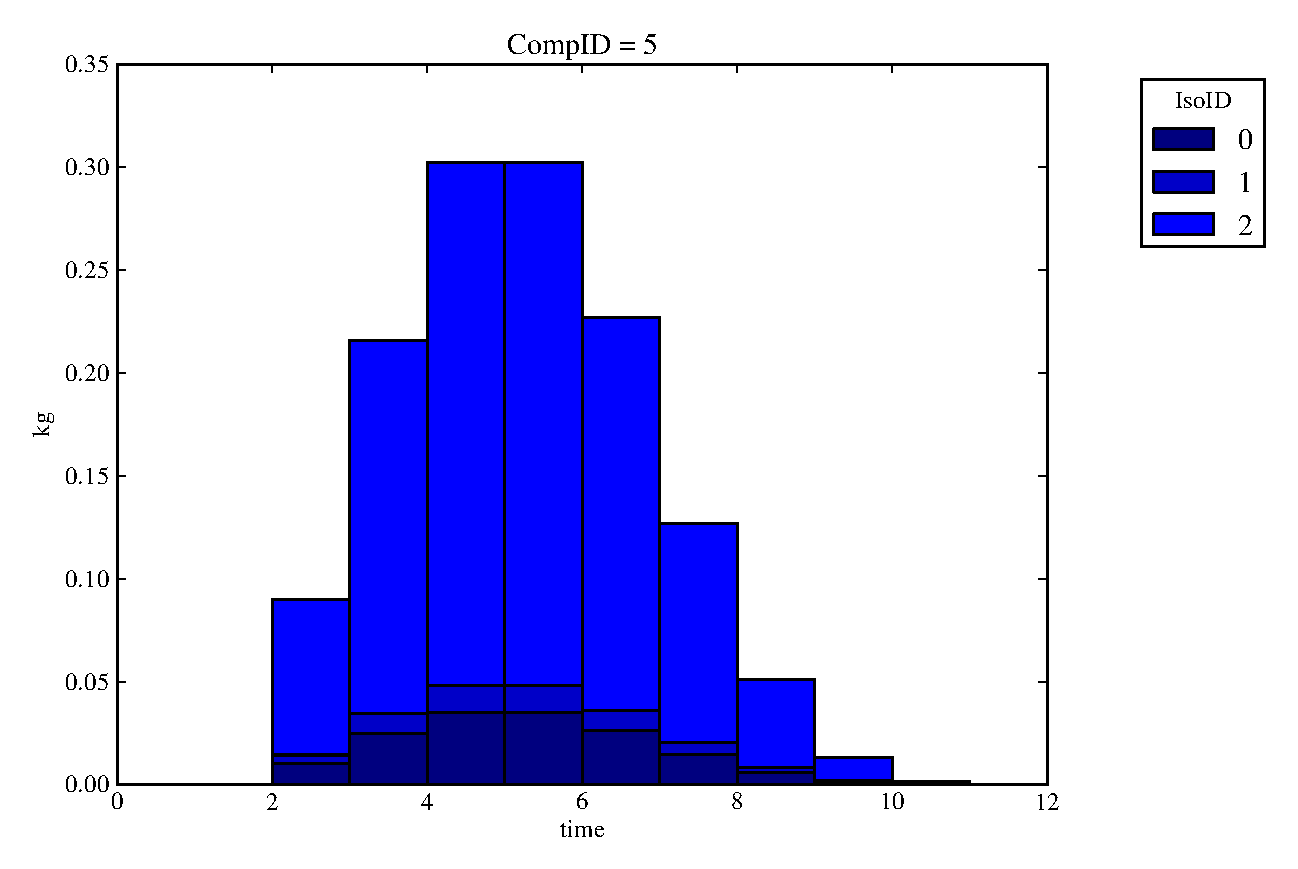
\includegraphics[width=0.2\textwidth]{cyder/images/buff0deg5.eps}
      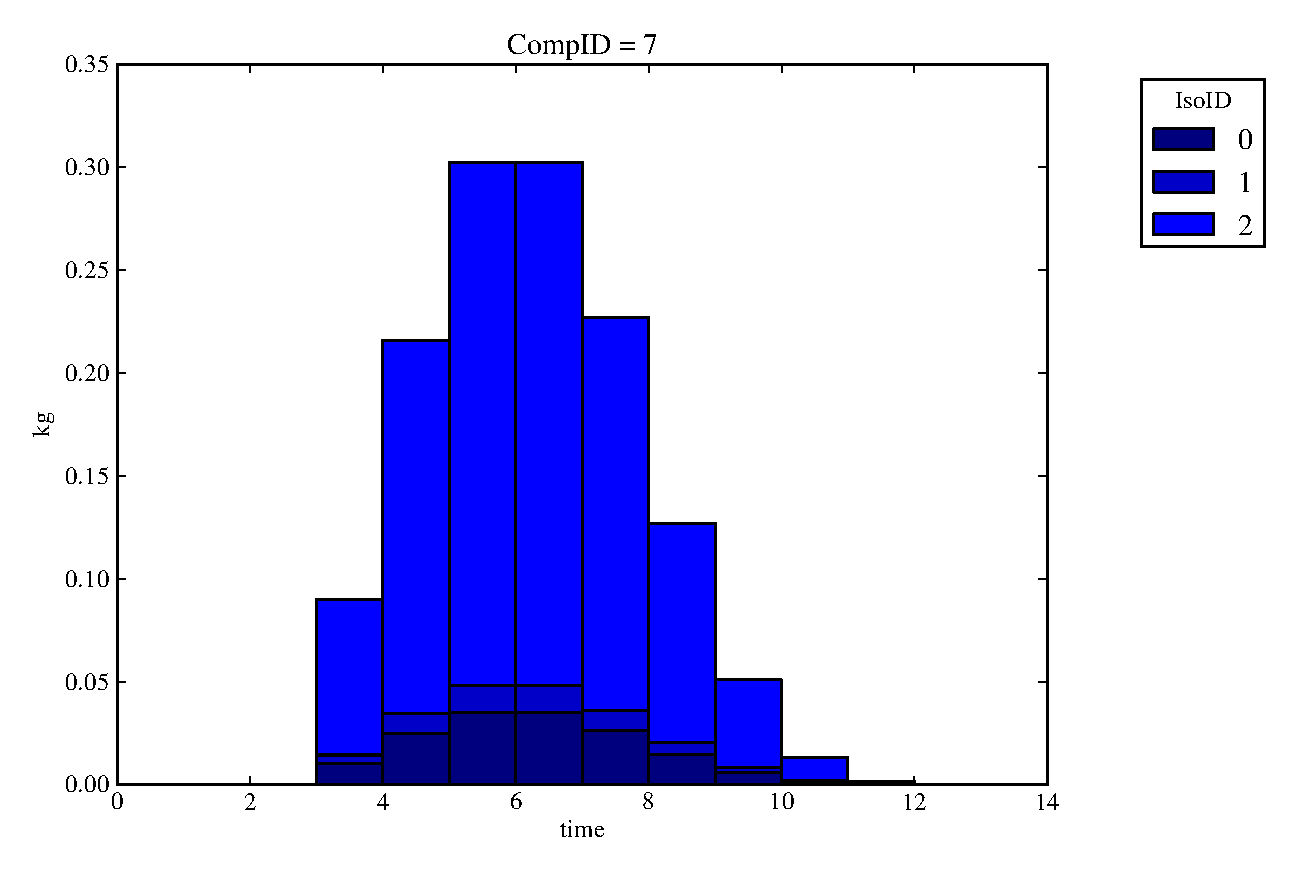
\includegraphics[width=0.2\textwidth]{cyder/images/buff0deg7.eps}
      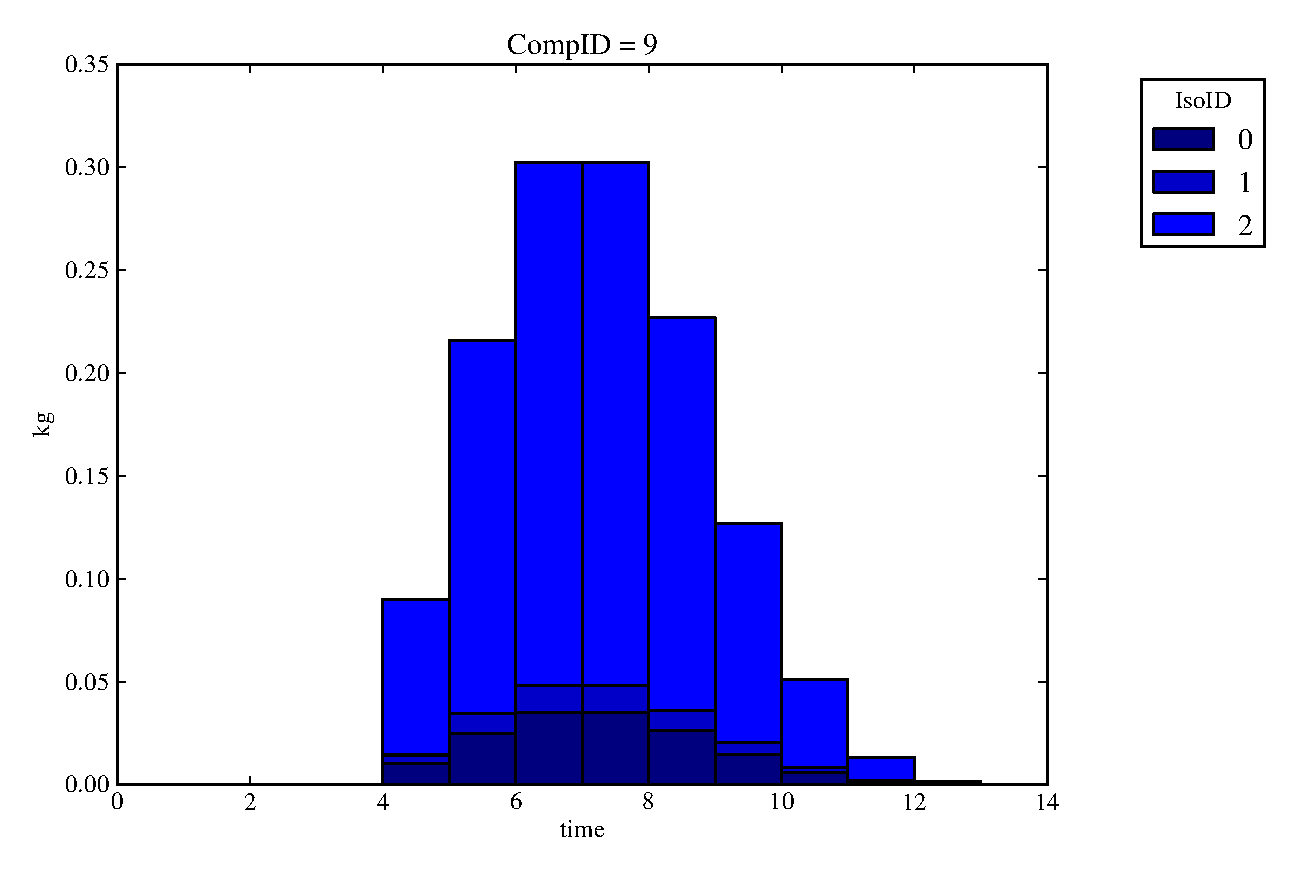
\includegraphics[width=0.2\textwidth]{cyder/images/buff0deg9.eps}
      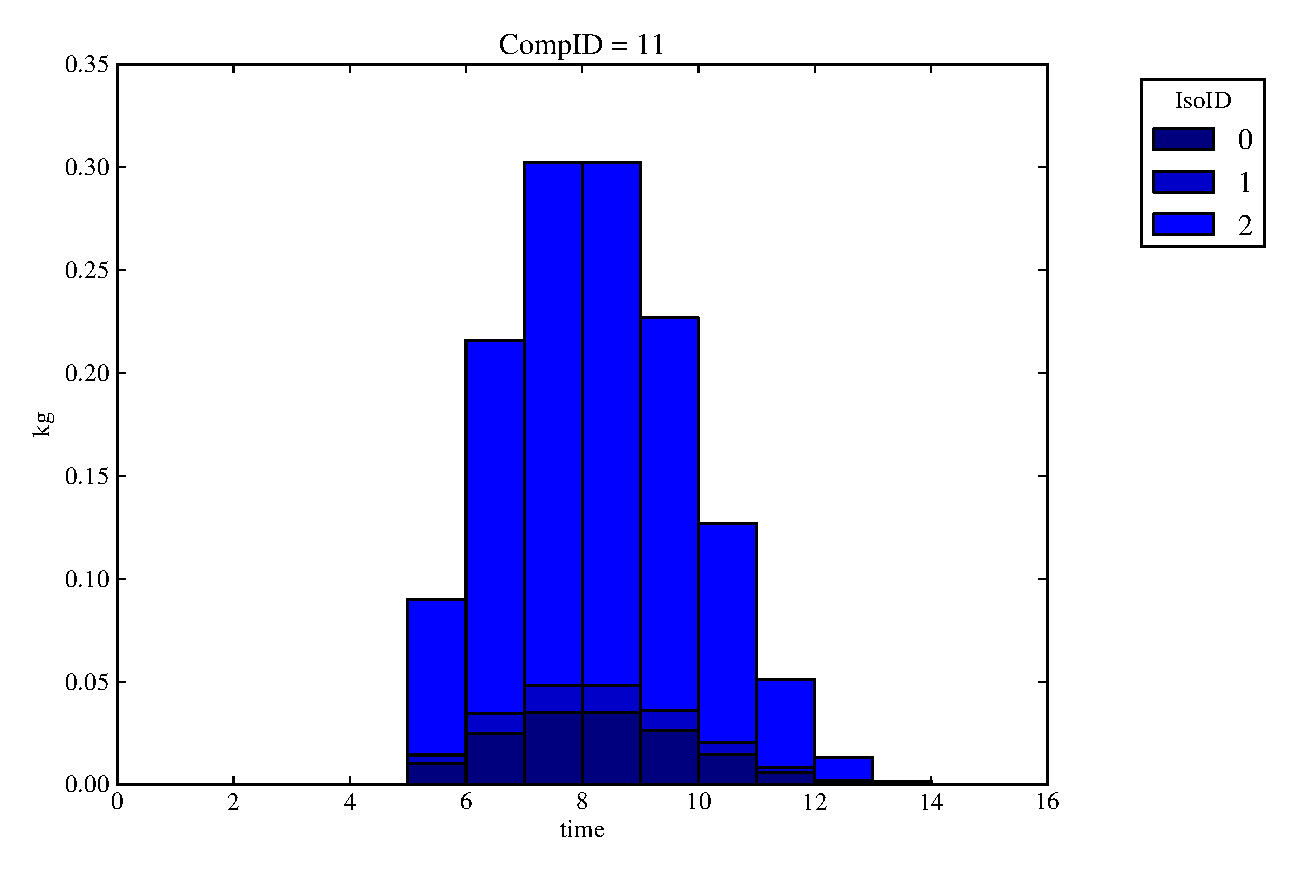
\includegraphics[width=0.2\textwidth]{cyder/images/buff0deg11.eps}
    \end{center}
  \end{figure}
\end{frame}

\begin{frame}
  \frametitle{Degradation Rate Base Case II}
  Base Case II : If the degradation rates for all pieces are 10\% per timestep 
  except the buffer. If five waste forms are necessary, the far field should 
  recieve no material within the 100 timesteps.

  \begin{figure}[htbp!]
    \begin{center}
      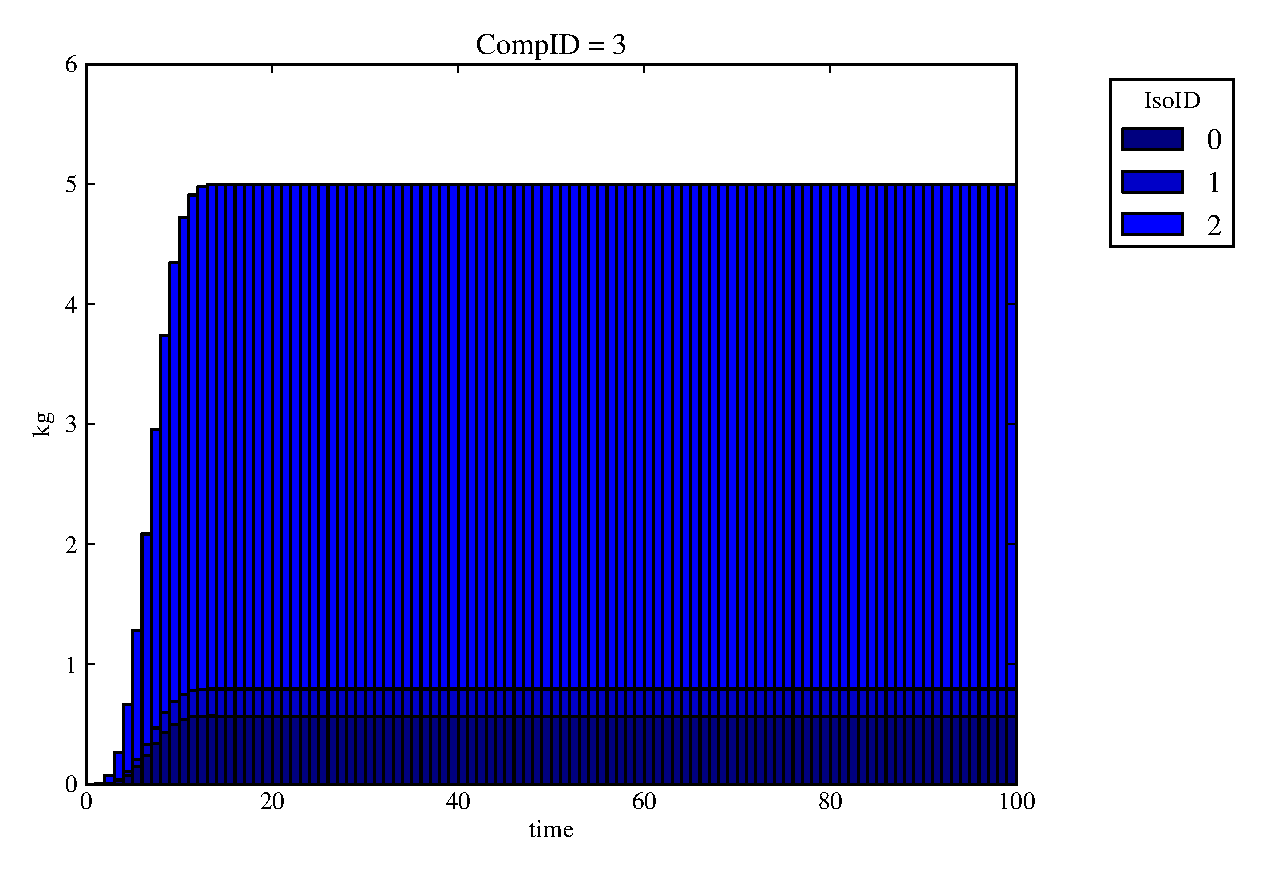
\includegraphics[width=0.5\textwidth]{cyder/images/buff0deg3.eps}
    \end{center}
  \end{figure}
\end{frame}

